\documentclass{article}

\usepackage{url} % Tidy web links
\usepackage{microtype} % 'Improved' typesetting
\usepackage{parskip} % Adds white space between paragraphs
\usepackage[super]{natbib} % Citations using superscript
%\usepackage{natbib} % Citations using superscript
\usepackage[a4paper, left=1.5cm, right=1.5cm, top=1.5cm, bottom=2.0cm]{geometry}
\usepackage{longtable,booktabs}  % For tables
\usepackage{caption} % For figure and table captions
\usepackage{graphicx} % Adds more functionality to graphics for inclusion of figures
\usepackage{lineno} % Allows use of \linenumbers to add line numbers 
\usepackage[toc,page]{appendix}
\usepackage[utf8]{inputenc}
\frenchspacing % No double spacing between sentences
\linespread{1.2} % Set linespace
\usepackage{authblk} % For author formatting
\usepackage{lmodern} % A scalable font - avoids erros due to non-sclabale fonts
\usepackage{subcaption} % Allows use of subfigures
\DeclareUnicodeCharacter{2060}{\nolinebreak} % Prevent unicode (U+2060) error on local complile
\usepackage{cclicenses} % For creative commons license
\usepackage{xcolor} % for coloured text
\usepackage{xurl} %for url but with more flexible linebreaking
\usepackage[hybrid]{markdown}

\renewcommand{\thefootnote}{\alph{footnote}} % Use letters for footnotes
\setcitestyle{square} % Refs in square brakcets



% Choose your own colour
\usepackage{color}
\newcommand{\mjanote}[2][\textcolor{red}{\dagger}]{\textcolor{red}{$#1$}\marginpar{\color{red}\raggedright\tiny$#1$ #2}}
\newcommand{\mjaFIXME}[1]{\textcolor{red}{[\textbf{FIXME} \textsl{#1}]}}
\newcommand{\kpnote}[2][\textcolor{magenta}{\dagger}]{\textcolor{magenta}{$#1$}\marginpar{\color{magenta}\raggedright\tiny$#1$ #2}}
\newcommand{\kpFIXME}[1]{\textcolor{magenta}{[\textbf{FIXME} \textsl{#1}]}}

\hbadness=1000000 % Turn off \hbox badness warnings

% Word counts
\usepackage{verbatim}

\newcommand{\detailtexcount}[1]{%
  \immediate\write18{texcount -sub=section -merge -sum -q #1.tex output.bbl > #1.wcdetail }%
  \verbatiminput{#1.wcdetail}%
}

\newcommand{\quickwordcount}[1]{%
  \immediate\write18{texcount -1 -sum -merge -q #1.tex output.bbl > #1-words.sum }%
  \input{#1-words.sum} words%
}

\newcommand{\quickcharcount}[1]{%
  \immediate\write18{texcount -1 -sum -merge -char -q #1.tex output.bbl > #1-chars.sum }%
  \input{#1-chars.sum} characters (not including spaces)%
}

\begin{document}
% Info on wordcounts:
% https://www.overleaf.com/learn/how-to/Is_there_a_way_to_run_a_word_count_that_doesn%27t_include_LaTeX_commands%3F

% To include refs in word count:
%TC:incbib

% Ignore title and abstract in word count
%TC:ignore
% Rewrite this title to include dementia

\title{STOKE-IMPACT: Understanding the impact of clinical practice variation on patient outcomes using explainable machine learning coupled with clinical trial emulation and causal inference studies. A study using national clinical audit data.}
\author{} % Hide author
\date{} % Hide date
\maketitle
\vspace{-20mm}
%TC:endignore


%\section*{Plain English Summary}

The focus of our team's work is on using explainable machine learning, clinical pathway simulation, and geographic modelling, applied to national clinical audit data to identify between-hospital variation in clinical decision-making and processes, and understanding the impact of that variation on patients and on the use of health service resources. Our work is in collaboration with the Sentinel National Stroke Audit Programme, and focuses mostly on the emergency stroke pathway, but is applicable across other clinical areas.

In our work we uncover potential causes of between-hospital variation. For example, in the use of clot-busting medication (\textit{thrombolysis}) in stroke, the majority of the large between-hospital variation in use of these drugs appears to come from differences in decision-making and in-hospital processes, rather than from differences in the characteristics of the patients attending each hospital. Another example is that appears early use of these clot-busting drugs reduces the risk of death even in mild strokes, but late use can increase the risk of death. These are important observations that may be used to advocate for change in clinical practice. Though our models attempt to isolate the effects of different factors, we would like to use multiple different methods to strengthen the \textit{cause-and-effect} conclusions from our current models. This will help rule out our current observations being coincidence (for example, if early use of clot-busting drugs is linked to a reduction in death, can we be sure this isn't just because the patients receiving treatment earlier have characteristics that make them less likely to die anyway?). We wish, for example, to confirm that early use of thrombolysis is actually causing the observed reduction in death. To do this we would use methods known as \textit{causal inference analysis}.

When using data that has been collected in routine clinical practice, no method is perfect for confirming a cause-and-effect, but by incorporating multiple methods into our analysis we wish to test our observations from our machine learning as much as possible. Example methods that might be used include \textit{target trial emulation} (where the patient set is restricted to those that have been through clinical trials in a similar area of study), or \textit{matching} where matched pairs of patients are found that are very similar apart from the one characteristic that we think may be important.

Adding methods that more directly investigate cause-and-effect will substantially strengthen our suite of tools. We have recently added \textit{explainability} to our machine-learning models (so that we can see what led to any particular prediction the model made). Adding stronger cause-and-effect analysis would help test our models further and build more trust in conclusions and recommendations made. 

The work will find immediate use in the various stroke modelling projects we undertake with the national stroke audit and with national and regional NHS organisations. During this project we will hold stakeholder workshops, to help develop the work so it is understable by, and useful for, stakeholders. This will use our existing stakeholder network across the Sentinel Stroke National Audit including the newly established NHS-England \textit{communities of practice of thrombolysis}, which bring together stroke teams with differing use of clot-busting drugs. We will also regularly involve patients and carers in discussing the work - our experience is that this very significantly helps test our knowledge on the models, and helps us to develop much clearer communication of the models and the results.

In addition to development of the methodology, this project will be used to develop the skills and capabilities of Kerry Pearn (co-PI) who will lead the project with assistance from Michael Allen (Co-PI). The stroke modelling and data science team is a stable team, funded by research grants and NHS-contracted work, and the techniques and skills developed here will find long-term use and benefit.
%\section{Plain English Summary}

\textbf{Aim}

Our aim is to improve the benefit that can be achieved from the use of the medical stroke treatment (\textit{thrombolysis}) for people who have had a stroke caused by a clot. This treatment is only available for the first few hours of stroke care. Currently there is a lot of variation between each hospital at providing this care. We currently use various modelling techniques to understand the impact of that variation on patients, and the impact on the use of resources in the health care setting. We would like to extend and strengthen our current work by using a number of \textit{causal inference methods}, with the aim to rule out our current observations being due to a coincidence. We would like to identify, with confidence, the cause-and-effect relationships. We will then be able to produce tailored guidance, for each hospital, about how they can improve their patient outcomes. 

We already have very strong direct links for how our findings will benefit patients. NHS-England will use our findings to support specific hospitals with their improvements, and the national stroke audit will incorporate our findings from spring 2024. The techniques and skills developed here will be used immediately in our other stroke care related projects, and will provide a huge benefit to many future projects. 

\textbf{Background to the research}

Stroke is one of the leading causes of death and disability. For every 10 strokes, 8 are caused by a clot in the brain. For these patients there is the possibility to reduce, or remove, the clot by use of thrombolysis (a medical stroke treatment). The use of thrombolysis varies a lot between hospitals, and the overall use is only about half of the NHS target. It has been stuck at this lower rate for nearly 20 years. Resources are currently available to set up new mechanisms to help hospitals improve. This includes the newly established NHS-England \textit{communities of practice of thrombolysis}, which brings together stroke teams with a large difference in their use of thrombolysis. Our modelling work can provide additional insight to this improvement process, by identifying the most effective change for each hospital. 

We have already identified some potential reasons for this variation in stroke care between different hospitals. For example, the largest reason comes from the different processes occurring at each hospital (including each hospital having their own way to decide which patient should receive the medical stroke treatment, \textit{thrombolysis}). Less variation is coming from the difference in the characteristics of the patients attending each hospital. Another useful insight from our modelling work shows that for people suffering a mild stroke, early use of thrombolysis appears to reduce the risk of death, but late use can increase the risk of death. These are important observations that may be used to support a change in clinical practice. However, our current models are not the right type for us to state any \textit{cause-and-effect} conclusions. There is a chance that any current observations are a coincidence. For example, if early use of thrombolysis is linked to a reduction in death, can we be sure this isn't just because the patients receiving treatment earlier have characteristics that make them less likely to die anyway? We wish, for example, to confirm that early use of thrombolysis is actually causing the observed reduction in death. To do this we would use methods known as \textit{causal inference analysis}. By extending our current work to using a number of \textit{causal inference methods}, we will strengthen our findings by ruling out any current observation being due to a coincidence.

\textbf{Design and methods used}

We work together with the Sentinel Stroke National Audit Programme. Our models are based on their detailed stroke dataset, that contains a record for each patient that has had a stroke. When we use data that has been collected as part of the daily hospital routine, no modelling method will be perfect for confirming a cause-and-effect. But by using a number of \textit{causal inference methods} we can test our observations as much as possible. The \textit{causal inference methods} that might be used include \textit{target trial emulation} (where patients are only included if they represent the type that were included in a relevant clinical trial), or \textit{matching} (where matched pairs of patients are found that are very similar apart from the one characteristic that we think may be important). We will hold stakeholder workshops that will help us to develop the work so that it is understandable by, and useful for, stakeholders. We will use our existing stakeholder network across the Sentinel Stroke National Audit, including the newly established NHS-England \textit{communities of practice of thrombolysis}.

\textbf{Patient and public involvement}

We regularly and consistently discuss our work with an engaged group of patients and carers. This process has previously helped us to have a clear way to communicate the models and the results, which in turn has improved our knowledge of the models. The patients and carers have also guided our work to look at what benefits patient outcomes, and not just about meeting arbitrary targets on thrombolysis use. The same process will continue for this project.

\textbf{Dissemination}

Our findings will be shared and used by the national stroke audit and NHS-England. Being published in the monthly stroke audit will also give the clinical stroke community easy access to our findings. We will also publish our work in leading stroke journals, and present it at stroke conferences. All of our detailed work is published online for anyone to freely access and use.
%\section*{Plain English Summary}

\textbf{Aim}

Our aim is to improve the benefit that can be achieved from the use of the medical stroke treatment (\textit{thrombolysis}) for people who have had a stroke caused by a clot. This treatment is only available for the first few hours of stroke care. There is a large variation between each hospital at providing this care. We currently use various modelling techniques to understand the impact of this variation on patients, and on the use of health care resources. We would like to extend and strengthen our work by using \textit{causal inference methods}, with the aim to rule out observations being due to a coincidence, and identify the cause-and-effect relationships. We will produce guidance for each hospital about how they can improve their patient outcomes. 

We already have strong direct links for how our findings will benefit patients. NHS-England will use our findings to support specific hospitals with their improvements, and the national stroke audit will incorporate our findings from spring 2024. The knowledge developed here will be used immediately in our other stroke care related projects, and will provide a huge benefit to many future projects. 

\textbf{Background to the research}

Stroke is one of the leading causes of death and disability. For every 10 strokes, 8 are caused by a clot in the brain. For these patients there is the possibility to reduce, or remove, the clot by use of thrombolysis. Thrombolysis use varies a lot between hospitals, and the overall use is only about half of the NHS target. Resources are currently available to create new mechanisms to help hospitals improve. This includes the newly established NHS-England \textit{communities of practice of thrombolysis}, which brings together stroke teams with a large difference in their thrombolysis use. Our modelling work can provide additional insight to this improvement process, by identifying the most effective change for each hospital.

Our models have already identified some potential reasons for this variation in stroke care between hospitals. One useful insight shows that for people suffering a mild stroke, early use of thrombolysis appears to reduce the risk of death, but late use can increase the risk of death. This important observation may be used to support a change in clinical practice. However, our current models are not the right type for us to state any \textit{cause-and-effect} conclusions. To be able to confirm that early use of thrombolysis is actually causing the observed reduction in death we would use \textit{causal inference analysis}. By extending our current work to using \textit{causal inference methods}, we will strengthen our findings by ruling out any current observation being due to a coincidence.

\textbf{Design and methods used}

Our models are based on the Sentinel Stroke National Audit Programme detailed stroke dataset. It contains a record for each patient that has had a stroke. No modelling method will be perfect for confirming a cause-and-effect relationship from routinely collected data. But by using a number of \textit{causal inference methods} we can best test our observations. The \textit{causal inference methods} that might be used include \textit{target trial emulation} (only included patients if they represent those that were included in a relevant clinical trial), or \textit{matching} (matched pairs of patients are included that are very similar apart from the one characteristic that may be important). We will hold stakeholder workshops to help us develop the work so that it is understandable by, and useful for, stakeholders. We will use our existing stakeholder network across the Sentinel Stroke National Audit, including the NHS-England \textit{communities of practice of thrombolysis}.

\textbf{Patient and public involvement}

We regularly discuss our work with an engaged group of patients and carers. This process has previously helped us to communicate the models and the results clearly, which in turn has improved our knowledge of the models. The patients and carers also guided our work to look at what benefits patient outcomes, and not just about meeting arbitrary targets. The same process will continue for this project.

\textbf{Dissemination}

Our findings will be shared and used by the national stroke audit and NHS-England. Being published in the monthly stroke audit will also give the clinical stroke community easy access to our findings. We will also publish our work in leading stroke journals, and present it at stroke conferences. All of our detailed work is published online for anyone to freely access and use.
\section{Research plan}

\subsection{What is the problem?}

Stroke remains one of the leading causes of death and disability, globally and in the UK. Thrombolysis with recombinant tissue plasminogen activator, can significantly reduce disability after ischaemic stroke, so long as it is given in the first few hours after stroke onset \cite{emberson_effect_2014}. Despite thrombolysis being of proven benefit in ischaemic stroke, use of thrombolysis varies significantly both between and within European countries \cite{aguiar_de_sousa_access_2019}. In England and Wales the national stroke audit reported that in 2021/22, 20 years on from the original European Medicines Agency licencing of alteplase for acute ischaemic stroke, thrombolysis rates for emergency stroke admissions varied from just 1\% to 28\% between hospitals \cite{sentinel_national_stroke_audit_programme_ssnap_2022}, with a median rate of 10.4\% and an inter-quartile range of 8\%-13\%, against a 2019 NHS England long term plan that 20\% of patients of emergency stroke admissions should be receiving thrombolysis.

Our research team uses various modelling techniques, including \textit{explainable machine learning} to identify the variation that occurs across different hospitals during the first few hours of stroke care. We use these models to understand the the source and impact of that variation on patients \cite{allen_using_2022, allen_use_2022}. We work together with the Sentinel Stroke National Audit Programme and NHS-England on reducing between hospital-variation in emergency stroke care. 

\subsection{Why is this research important?}

Variation in use of thrombolysis in emergency stroke care is hampering the ability to meet NHS targets on use of this disability-saving treatment, and is causing inequality of access to this treatment. 

Thrombolysis rates are, however, only half the story. As thrombolysis also carries a risk of serious injury, it is important to check that improving thrombolysis rates will improve outcomes.

The planned work seeks to add causal inference methodologies to our methods - to strengthen the trust that changes suggested would indeed lead to improved outcomes.

\subsection{Review of existing evidence}

% 1) What is the problem?


% 2) What do we know about low and varying use of thrombolysis

Studies have shown that reasons for low and varying thrombolysis rates are multi-factorial. Reasons include late presentation \cite{aguiar_de_sousa_access_2019}, lack of expertise \cite{aguiar_de_sousa_access_2019} or lack of clear protocols or training \cite{carter-jones_stroke_2011}, delayed access to specialists \cite{kamal_delays_2017}, and poor triage by ambulance or emergency department staff \cite{carter-jones_stroke_2011}. For many factors, the establishment of primary stroke centres has been suggested to improve the emergency care of patients with stroke and reduce barriers to thrombolysis \cite{carter-jones_stroke_2011}, with a centralised model of primary stroke centres leading to increased likelihood of thrombolysis \cite{lahr_proportion_2012, morris_impact_2014, hunter_impact_2013}. 

In addition to organisational factors, clinicians can have varying attitudes to which patients are suitable candidates for thrombolysis. In a discrete choice experiment \cite{de_brun_factors_2018}, 138 clinicians considered hypothetical patient vignettes, and responded as to whether they would give the patients thrombolysis. The authors concluded that there was considerable heterogeneity among respondents in their thrombolysis decision-making. Areas of difference were around whether to give thrombolysis to mild strokes, to older patients beyond 3 hours from stroke onset, and when there was pre-existing disability.

Based on national audit data from three years of emergency stroke admissions, we have previously built models of the emergency stroke pathway using clinical pathway simulation to examine the potential scale of the effect of changing two aspects of the stroke pathway performance (1. the in-hospital process speeds, and 2. the proportion of patients with a determined stroke onset time), and using machine learning to examine the effect of replicating clinical decision-making around thrombolysis from higher thrombolysing hospitals to lower thrombolysing hospitals \cite{allen_using_2022, allen_use_2022}. The machine learning model, which has 85\% accuracy (ROC-AUC = 0.92), learned whether any particular patient would receive thrombolysis in any particular emergency stroke centre. Using these models we found that it would be credible to target an increase in average thrombolysis in England and Wales, from 11\% to 18\%, but that each hospital should have its own target, reflecting differences in local populations. We found that the largest increase in thrombolysis use would come from replicating thrombolysis decision-making practice from higher to lower thrombolysing hospitals. Two other important factors influencing thrombolysis rates were determination of stroke onset time in some hospitals, and improving the speed of the in-hospital thrombolysis pathway.

We have extended the model to including explainability \cite{pearn_what_2023} (see figure \ref{fig:shap}). This revealed that lower thrombolysing hospitals, compared with higher thrombolysing hospitals, were particularly less likely to give thrombolysis to patients with 1) mild stroke, 2) imprecisely known onset time, 3) patient with prior disability, 4) any combination of those.

\begin{figure}
\centering
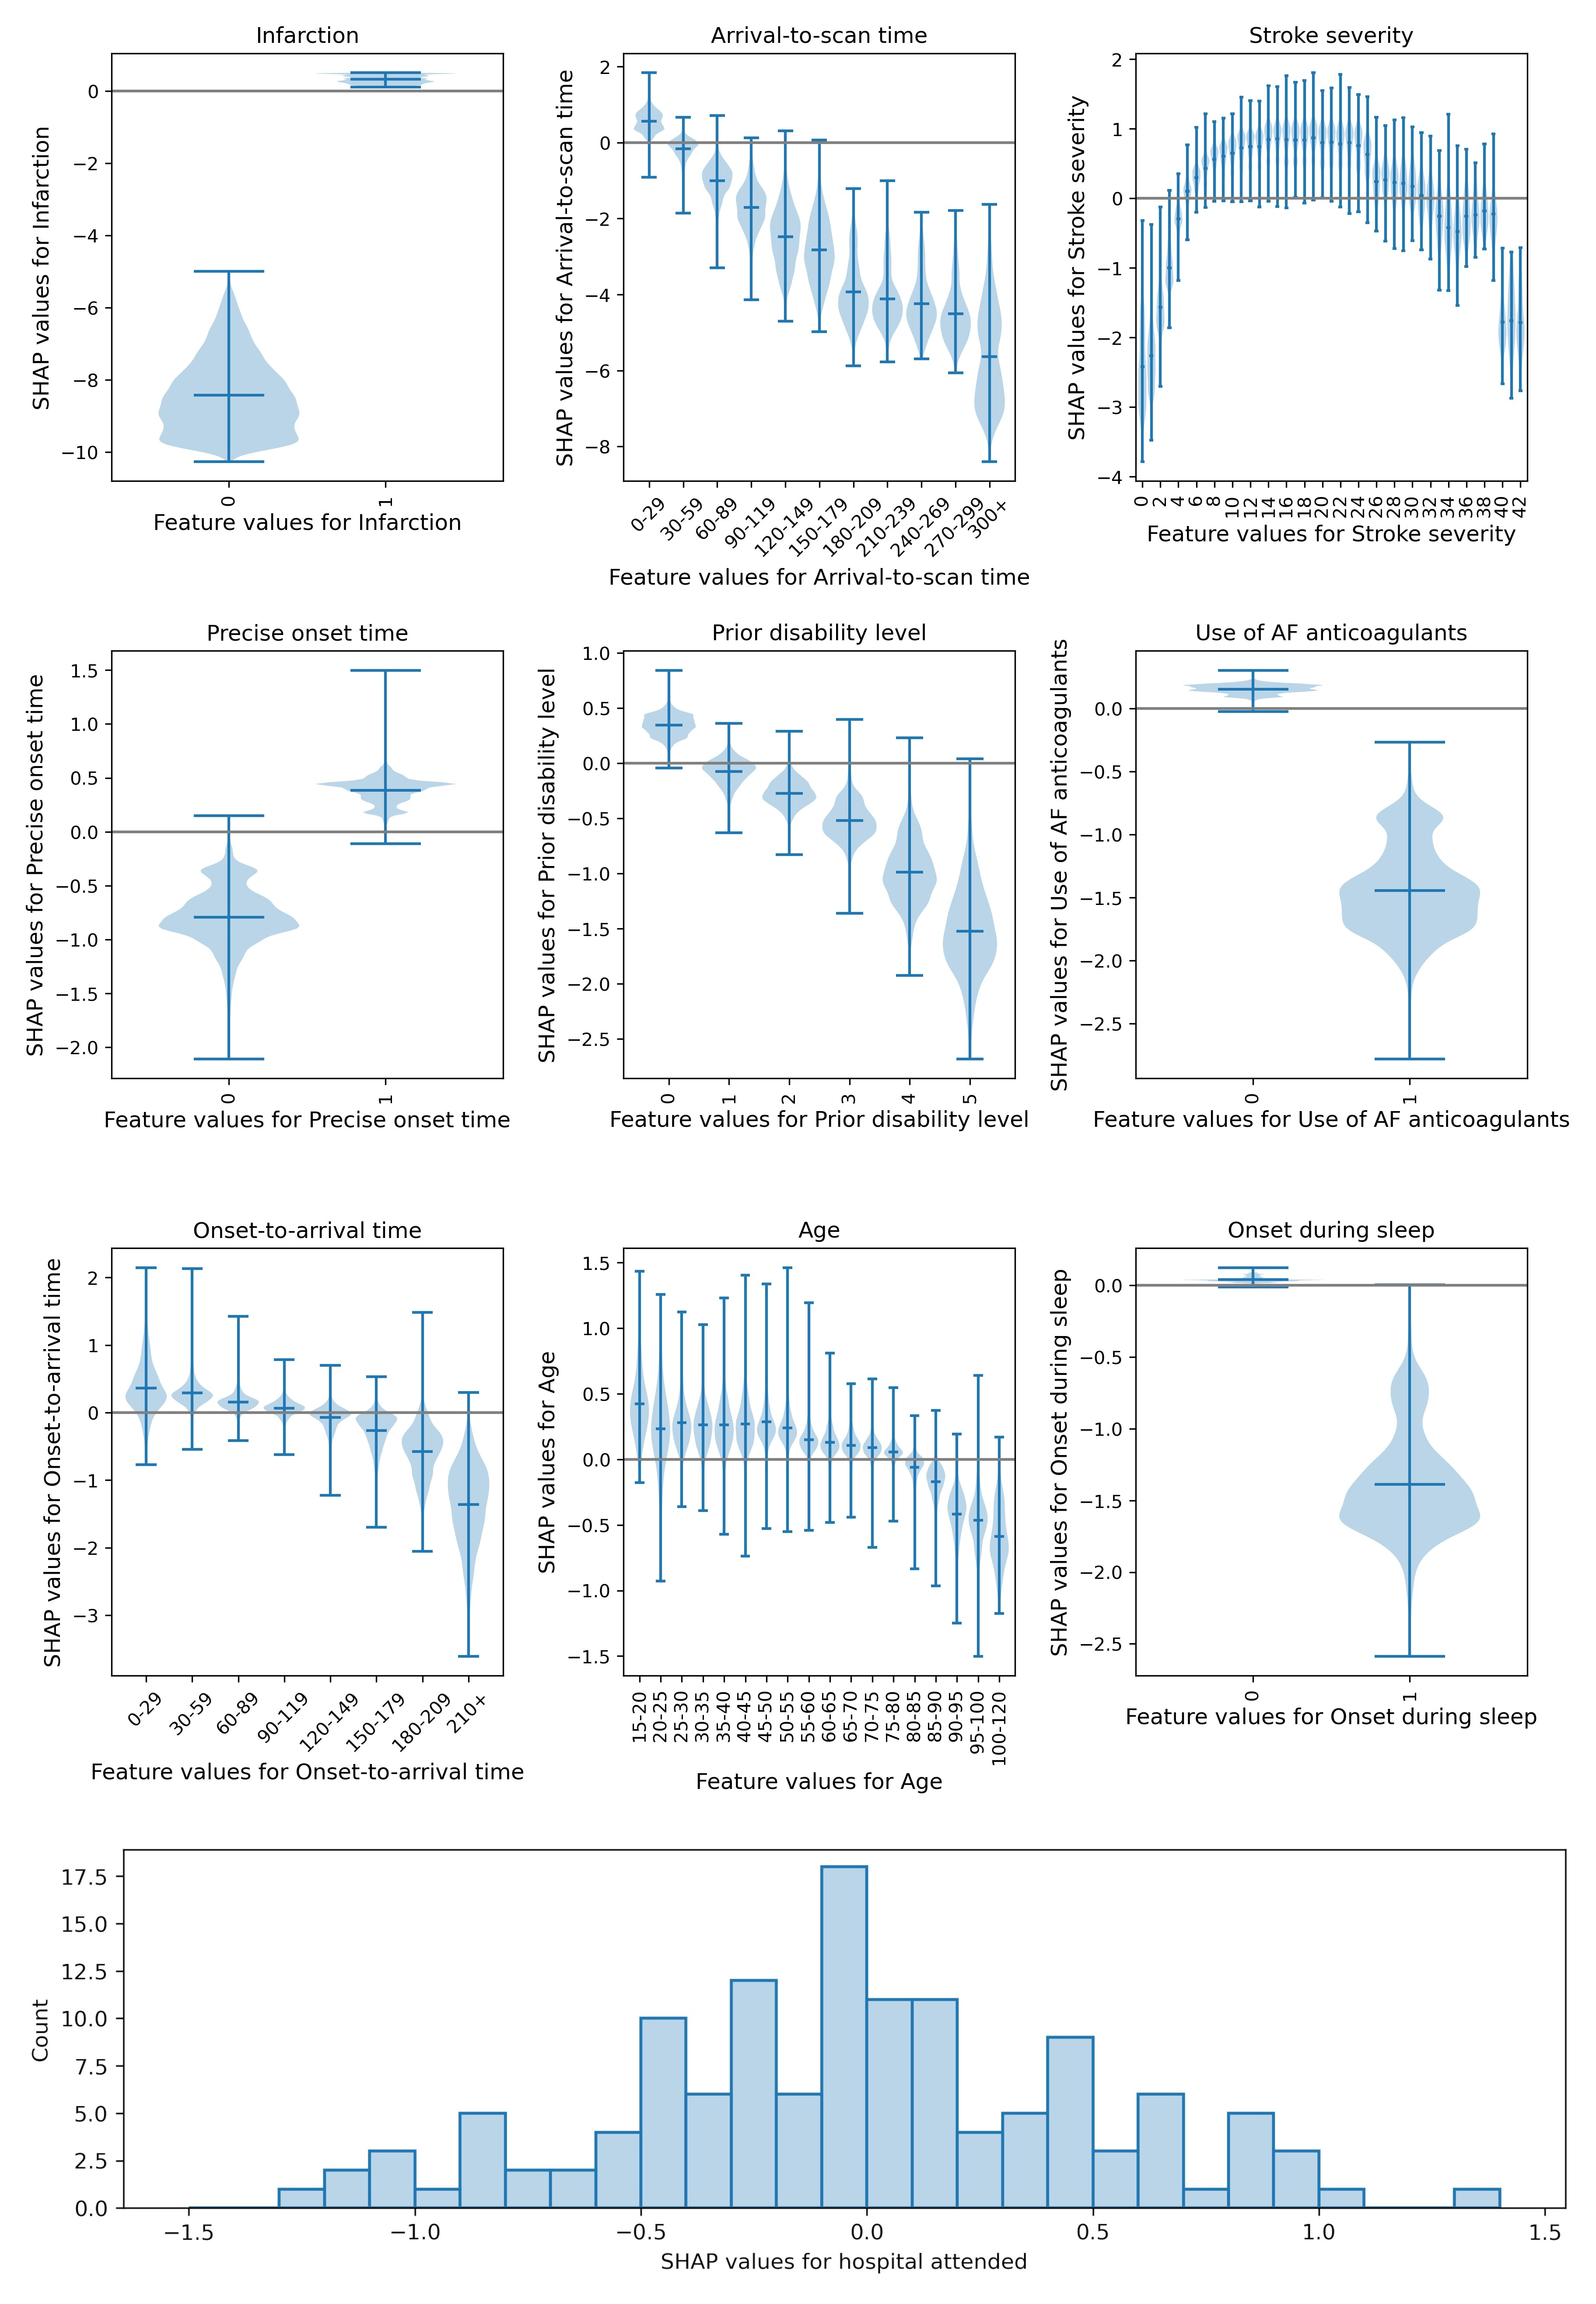
\includegraphics[width=0.85\textwidth]{./images/combined_shap}
\caption{Plots showing the relationship between feature values and how the log-odds of receiving thrombolysis are effected (the \textit{SHAP} value). Top: Violin plots showing the relationship between SHAP values and feature values. The horizontal line shows the median SHAP value. The plots are ordered in ranked feature importance (using the mean absolute SHAP value across all instances). Bottom: Histogram showing the frequency of SHAP values for the hospital attended.}
\label{fig:shap}
\end{figure}

We are developing a web app (available at \url{https://stroke-predictions.streamlit.app/} that allows teams to see how changing pathway process speeds, or changing decision-making, may change thrombolysis use and outcomes.


% 3) What do we not know

Current NIHR-funded work \footnote{https://fundingawards.nihr.ac.uk/award/NIHR134326} is focussing on building explainable machine learning models to predict death and disability-level outcomes with and without thrombolysis (and with differing time to thrombolysis). The observational data set we are using has over 40,000 patients receiving thrombolysis, compared to 6,756 in the seminal meta-analysis conducted by Emberson \textit{et al.} \cite{emberson_effect_2014}. Use of observational data also allows the investigation of the effect of thrombolysis as use is extended outside of clinical trial inclusion criteria. 

Some patterns are appearing in the analysis which may help guide clinicians on use of thrombolysis. In mild stroke (which was not generally included in the clinical trials), we observe that early thrombolysis is associated with a reduced chance of death, whereas later thrombolysis is associated with an increased chance of death (fig \ref{fig:death}). It is possible, however, that this effect is co-incidental rather than causal. We therefore wish to strengthen this type of analysis, by combining explainable machine learning with a range of causal inference methods.

\begin{figure}
\centering
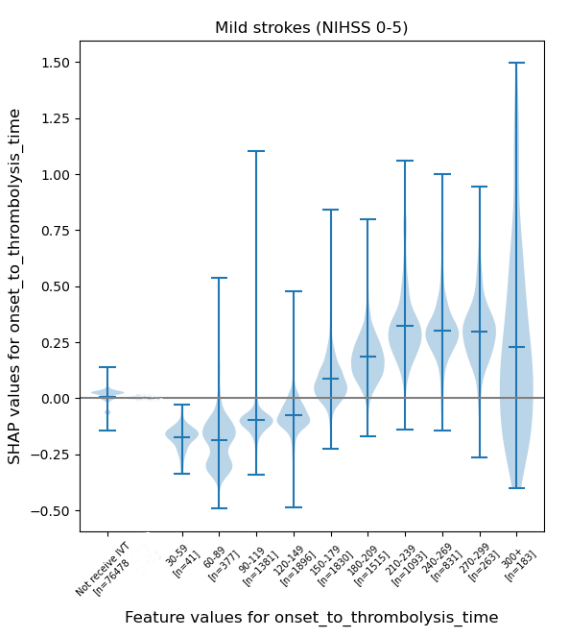
\includegraphics[width=0.5\textwidth]{./images/death}
\caption{Violin plot showing the relationship between time to thrombolysis and and how the log-odds of death are effected (the \textit{SHAP} value) in mild strokes (NIHSS 0-5).}
\label{fig:death}
\end{figure}

\subsection{Research aims}

The key aim of the proposed research is to incorporate causal inference methodology into our clinical pathway simulation and explainable machine learning analysis of emergency stoke care. We consider this a key methodological development, alongside explainable machine learning, to test, and build trust in, how changes in use of thrombolysis will effect outcomes.

\subsubsection{Specific research questions}

We are interested in incorporating causal inference analysis into a wide range of our work, but he have specific research questions to pin this development to. These research questions will help ensure advice given to stroke teams has the strongest foundations for improving outcomes.

\begin{itemize}
    \item In subgroups of patients where we see significant inter-hospital variation in use of thrombolysis, is there good evidence that the hospital is causing the variation in thrombolysis use in these groups (rather than this effect coinciding with other factors)? Example patient subgroups are 1) Mild stroke (at presentation), 2) Presence of prior disability, and 3) Imprecisely known stroke onset time.

    \item In subgroups of patients where we see significant changes in outcome, is there good evidence that the main feature of interest in the patient subgroup is causing the variation in outcome in these groups (rather than this effect coinciding with other factors)? Example patient subgroups include early vs. late thrombolysis in mild stroke (where early thrombolysis appears to reduce the odds of death, but late thrombolysis increases the odds of death)?
\end{itemize}


\subsection{Project plan}

\subsubsection{Data}

We use anonymous patient-level data from the Sentinel Stroke National Audit Programme (SSNAP, \url{https://www.strokeaudit.org/}. SSNAP collects data on essentially all emergency stroke units, from all stroke units in England, Wales, and Northern Ireland. The data includes a wide range of information such as data on times throughout the stroke pathway from stroke onset, pre-stroke disability (modified Rankin Scale, mRS), a breakdown of stroke symptoms using the NIHSS stroke scale, reperfusion treatment given (and timing), comorbidities, death in hospital, disability at discharge from inpatient care, and 6 month follow-up disability (the latter is complete for about 35\% of discharged patients). Data is collected for about 85,000 patients each year, 10-11\% of whom receive thrombolysis.

\subsubsection{Methods}

When using observational data, no single method can provide proof of causality. Instead we will use a series of methods, each of which will contribute to understand causality. These methods will be applied to choice of thrombolysis, and outcomes, especially where we have identified high between-hospital variation in the use of thrombolysis. 

\begin{itemize}

    \item \textbf{Explainable machine learning with SHAP} \cite{aas_explaining_2020} - We will continue to use SHAP analyse to provide machine learning models at a global level and for individual predictions.

    \item \textbf{DAG (directed acyclic graphs)} \cite{tennant_use_2021} - Articulating proposed causal relationships through use of DAGs help to make assumed or hypothesised causal and non-causal relationships clear. They are easily understood by non-technical audiences, and so form an excellent basis for discussions and workshops to explore proposed causal relationships with clinical experts. We will use these, alongside results from other methods, in co-production workshops.
    
    \item \textbf{Target trial emulation} \cite{bigirumurame_current_2023} - This method involves mimicking the original thrombolysis clinical trials from observational data, using the original trial inclusion criteria, and then extending to groups that were not included in the original trial.

    \item \textbf{Natural experiments} \cite{craig_natural_2017} - Natural experiments compare outcomes when changes in services in any hospital are known to have occurred. We may, for example, look for shifts in thrombolysis use in individual hospitals and investigate outcomes.

    \item \textbf{Covariate adjustment} \cite{igelstrom_causal_2022} - We will identify all of the potential confounding variables, and include all of them that we can in a predictive model. Confounders are features, such as stroke severity, that affect both the probability of receiving thrombolysis, and the patient outcome. 

    \item \textbf{Use of propensity score as an adjusting feature} \cite{rosenbaum_central_1983} - \textit{`Propensity'}, the likelihood of a person receiving thrombolysis (estimated from a separate machine learning model), is added to the outcome prediction model, allowing the outcome model to adjusted for patients' suitability for treatment. This helps to identify, and correct for, better outcomes occurring in patients suitable for thrombolysis, even if they did not receive thrombolysis.

    \item \textbf{Matching} - Creation of matched populations of control and test patients. Matching attempts to create cohorts of patients that are similar in both groups apart from the feature with proposed causal influence, allowing for an estimation of the effect of the causal feature under study. Matching may be performed using nearest-neighbour approaches \cite{stuart_matching_2010} or by propensity scores \cite{rosenbaum_central_1983}.

    \item \textbf{Stratification of results by propensity score} \cite{rosenbaum_central_1983} - allowing comparisons of groups of patients who have similar suitability for treatment with thrombolysis.

    \item \textbf{Instrumental variable analysis} \cite{stel_instrumental_2013} - This method compares outcomes depending on an 'instrument' that does not directly effect outcome, but effects the proposed causal feature. In our current model we isolate how a hospital affects the likelihood that a patient will be given thrombolysis; we will test this as an instrument to investigate whether there is a relationship between this feature and outcomes. This could provide a novel link between advanced explainable machine learning methods and causal inference work.
           
    \item \textbf{Inverse propensity weighting} \cite{glynn_introduction_2010} - Weighting the contribution of patients to the final outcome measurement based on their likelihood of receiving, or not-receiving, thrombolysis. This method gives most weight to patients who received thrombolysis, who are more like patients who usually do not receive thrombolysis (and \textit{vice versa}). It also gives more weight to patients who are borderline in whether they would receive treatment or not.   
       
    \item \textbf{Double machine learning} \cite{chernozhukov_doubledebiased_2017} - This method combines two machine learning models, one to predict use of treatment and the other to predict outcome from that treatment. The treatment model estimates the probability of treatment given the observed covariates, while the outcome model estimates the expected outcome given the observed covariates and treatment. The errors (residuals) in the models are used as surrogates for missing information in each models. This method isolates a features causal relationship with the outcome by fitting the residuals of the feature prediction to the residuals of the outcomes.
\end{itemize}

All work will be performed in Python using established libraries for each of the methods (especially the \textit{XGBoost}, \textit{SHAP}, \textit{DoWhy} and \textit{EconML} libraries). Work will be conducted in \textit{Jupyter notebooks}, all of which will be published in an online \textit{Jupyter Book}.

\subsubsection{Co-production with the NHS, and link to patient benefit}

During this project we will hold stakeholder workshops to obtain feedback on the work. This will use our existing stakeholder network across the SSNAP, Integrated Stroke Delivery Networks (ISDN) and Integrated Care Systems (ICS). As we are working alongside NHS-England and NHS-Elect with teams with low thrombolysis (see paragraph below), we will also use this experience to refine project outputs.

A pilot web portal is being made available from autumn 2023, providing analysis of thrombolyis use at each hospital, comparing decisions made to other hospitals, and providing modelling how changing process speeds or clinical decisions would likely effect thrombolysis use and outcomes (based on a mathematical model of outcome depending on time to thrombolysis).

The modelling work currently being performed\footnote{https://fundingawards.nihr.ac.uk/award/NIHR134326}) is planned to be incorporated into the national stroke audit from Spring 2024. This will provide teams with realistic target thrombolysis use for their own patient population, and identify which area of the stroke pathway to focus on (for example pathway speed, ascertainment of stroke onset time, thrombolysis decision making). Additionally, NHS-Elect (who are working with NHS-England, the SAMueL team, and the national stroke audit) have an NHS improvement target to “Improve access to thrombolysis such that by the end of 2027/28, 20\% of stroke patients will receive thrombolysis treatment”. This collaborative will be working with 6 low-thrombolysing teams in the first instance, before extending work to all emergency stroke teams. As part of the quality improvement work, the SAMueL team will be providing modelling on use of thrombolysis, including on variation in decision-making between hospitals. We consider it important that this work should, if at all possible, include strengthened work on causality (the links between changes to pathway and decision making, through to thrombolysis use, and through to outcome) so that we have greater confidence that changes suggested (and potentially made) will lead to the expected improvement in thrombolysis use and, most importantly, in better outcomes and not 'just' increased thrombolysis use.

\subsubsection{Dissemination}

In addition to working with the national stroke audit and stroke teams directly (see above), we will also publish our work in leading stroke journals, and present it at stroke conferences. All of our detailed work is published online (e.g. see \url{https://samuel-book.github.io/samuel_shap_paper_1}).

\subsubsection{Project team}

The project teams bring together experience of stroke care, machine learning, epidemiology, clinical trials, and causal inference work.

\begin{itemize}

    \item \textbf{Michael Allen (Co-PI, 25\% FTE)} co-leads our NIHR funded work on explainable machine learning \footnote{https://fundingawards.nihr.ac.uk/award/NIHR134326}, with a focus on the technical aspects of the project. Dr Allen has extensive experience of health systems modelling and machine learning.

    \item \textbf{Kerry Pearn (Co-PI, 50\% FTE)} has been the principal developer of our explainable machine learning methodology for prediction of thrombolysis use and outcome. Ms Pearn will co-lead the proposed work, with a focus on detailed work planning and execution, bringing in advice from co-investigators.

    \item \textbf{Martin James (Co-I, 5\% FTE)} is a stroke consultant and clinical director of the national stroke audit. Prof James co-leads our NIHR funded work on explainable machine learning \footnote{https://fundingawards.nihr.ac.uk/award/NIHR134326}, with a focus on clinical oversight of the project. Prof James will provide clinical oversight for this proposed project.

    \item \textbf{Mark Kelson (Co-I, 5\% FTE)} is a statistician working in the overlap between clinical trials, medical statistics, causal inference, reproducibility and data science. Prof Kelson will advise on statistics and causal inference methods.

    \item \textbf{João Delgado (Co-I, 10\% FTE)} is an epidemiologist focussing on management of conditions affecting cognitive function in old age, using traditional and modern epidemiology and statistical tools to analyse large datasets of electronical health records. Dr Delgado will advise on epidemiological methodologies such as use of propensity scores..

    \item \textbf{Lauren Asare (Researcher, 5\%)} is a research assistant in the University of Exeter PenARC Public and Patient involvement group. Ms Asare supports our stroke PCI team (which is chaired bya stroke survivor).

\end{itemize}

\subsubsection{Patient and carer involvement}

Our team has a dedicated PPI group who provide constant input into our work and have provided input to this bid. The PPI group have been a key voice in guiding our work to look at what maximises patient outcomes, and not arbitrary targets on thrombolysis use. The PPI team is chaired by Leon Farmer, a stroke supervisor, with guidance from Lauren Asare of the University of Exeter PenARC PPI team.

\subsubsection{People development}

In addition to development of the methodology, this project will be used to develop the skills and capabilities of Kerry Pearn (Co-PI) who will lead the project with assistance from Michael Allen (Co-PI). The stroke modelling and data science team is a stable team, funded by research grants and NHS-contracted work, and the techniques and skills developed here will find long-term use and benefit.

\subsubsection{Contribution beyond this project}

We work on a range of projects that would benefit from this method development in our work. For example, ee are working on stroke projects focussing on the pre-hospital pathway\footnote{https://fundingawards.nihr.ac.uk/award/NIHR202361} and the use of mobile stroke units\footnote{https://fundingawards.nihr.ac.uk/award/NIHR153982}. The methodological development above will add value to both of these, and also to other similar, projects. For example, it has previously been assumed that outcome from hemorrhagic stroke (the 20\% of strokes that are caused by a bleed rather than a clot) is independent of ambulance travel time, but some recent clinical trials on taking stroke patients further, to a hospital with more capabilities for stokes caused by clots, have suggested this may not be true. Using methods such as clinical trial emulation and our large database of stroke data we will have the potential to enhance our pre-hospital stroke care model to better model outcomes of haemorrhagic strokes with alternative pre-hospital pathways.

\subsection{Intellectual property}

We work on a principal that public funding should give public benefit, and so all our detailed work (code) is shared with an Open Licence, allowing anyone to use or develop it.


%\section{Bid Info}

\url{https://www.nihr.ac.uk/funding/rfpb-under-represented-disciplines-and-specialisms-highlight-notice-methodologists/33231}

\begin{markdown}

* Call opens – 17 May 2023    \item Expression of Interest - (500 words) 16 August 2023 at 1pm
* Close call – 13 September at 1pm
* Stage 1 outcome – December 2023
* Stage 2 call close - end of January 2024
* Stage 2 outcome – May 2024
* Start - September 2024?

## What does RfPB cover?

* Research into the provision and use of NHS services.
* Effectiveness and cost effectiveness evaluations of interventions.
* Research that examines the resource use of alternative means for healthcare delivery.
* Feasibility research to support applications for major awards to other funders.
* Development and refining of new interventions, scales or outcome measures.
*  Research to explore the potential for improving patient health and wellbeing through needs assessments, methods development and exploratory studies.
* Evidence synthesis and systematic reviews
\end{markdown}

%\begin{markdown}
# Background
\end{markdown}

%\section{Method development}


%\markdownInput{sections/9_stuff_to_inlcude.md}

%TC:ignore
\newpage
\bibliographystyle{naturemag}
\footnotesize
\bibliography{references}
%TC:endignore


%%TC:ignore
\section*{Word count}
%\quickwordcount{main}
\detailtexcount{main}
%TC:endignore


\end{document}


